\documentclass[tikz,multi]{standalone}
\providecommand*{\xMin}{}%
\providecommand*{\xMax}{}%
\providecommand*{\yMin}{}%
\providecommand*{\yMax}{}%
\renewcommand*{\xMin}{0}%
\renewcommand*{\xMax}{4}%
\renewcommand*{\yMin}{0}%
\renewcommand*{\yMax}{4}%
\begin{document}
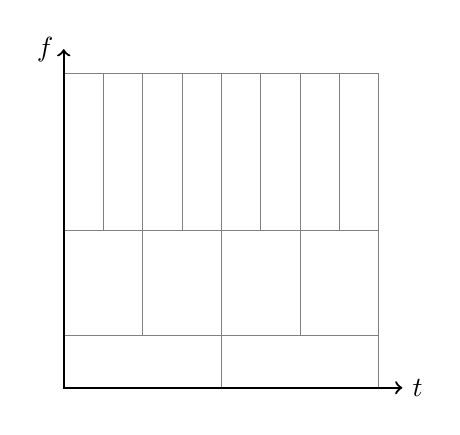
\begin{tikzpicture}
  \draw [very thin,gray] (\xMax,\yMin) -- (\xMax,4)  node [below] at (0,1){};
%First block (low resolution)
%h
  \draw [very thin,gray] (\xMin,0.666) -- (\xMax,0.666)  node [below] at (0,1){};
%h
  \draw [very thin,gray] (\xMin,2) -- (\xMax,2)  node [below] at (0,1){};
  % \draw [very thin,gray] (\xMin,1) -- (\xMax,1)  node [below] at (0,1){};
  \draw [very thin,gray] (2,0) -- (2,1)  node [below] at (2,0){};
%h
  % \draw [very thin,gray] (\xMin,2) -- (\xMax,2)  node [below] at (0,1){};
%v
  \draw [very thin,gray] (1,0.666) -- (1,2)  node [below] at (2,0){};
  \draw [very thin,gray] (2,0.666) -- (2,2)  node [below] at (2,0){};
  \draw [very thin,gray] (3,0.666) -- (3,2)  node [below] at (2,0){};
%h
  \draw [very thin,gray] (\xMin,4) -- (\xMax,4)  node [below] at (0,1){};
%v
  \draw [very thin,gray] (0.5,2) -- (0.5,4)  node [below] at (2,0){};
  \draw [very thin,gray] (1,2) -- (1,4)  node [below] at (2,0){};
  \draw [very thin,gray] (1.5,2) -- (1.5,4)  node [below] at (2,0){};
  \draw [very thin,gray] (2,2) -- (2,4)  node [below] at (2,0){};
  \draw [very thin,gray] (2.5,2) -- (2.5,4)  node [below] at (2,0){};
  \draw [very thin,gray] (3,2) -- (3,4)  node [below] at (2,0){};
  \draw [very thin,gray] (3.5,2) -- (3.5,4)  node [below] at (2,0){};

  \draw [<->,thick] (\yMin,\yMax + 0.3) node (yaxis) [left] {$f$}
    |- (\xMax + 0.3,\xMin) node (xaxis) [right] {$t$};
\end{tikzpicture}
\end{document}
